\chapter{绪论}\label{cha:intro}
本章首先阐述论文的选题背景和意义(\ref{sec:background}节);随后介绍与工作流网相关的预备知识(\ref{sec:preliminaries}节);\ref{sec:contribution}节给出论文的主要贡献;最后\ref{sec:structure}节介绍论文的章节安排。

\section{选题背景和意义}\label{sec:background}
如今信息系统需要支持业务过程的执行,而不是像以往一样仅仅关注于独立的任务。信息系统需要控制、监控并且支持一个业务过程逻辑层面的全部内容,即它应该能管理组织内的工作流。很多拥有大量业务过程的组织和企业对工作流的管理有着极为迫切的需求,这正是工作流管理兴起的原因\cite{van1998application}。在工作流管理技术的帮助下,企业可以快速建立或者更新自身的过程感知信息系统\cite{dumas2005process}。企业可以根据市场变化或者政府政策变更等外部因素随时调整自己的业务过程从而及时地改善自身的服务以提高企业的市场竞争力。

过程感知信息系统是由实际业务过程模型驱动的,这些模型描述了企业中的业务执行过程,每个任务的负责人以及需要的资源和产生的数据等。由于同一个业务过程可以被不同拓扑结构的图形所表示,因此它的行为语义才是刻画该过程的本质特征。任务间有序关系\cite{esparza2002improvement}常常被用来描述业务过程的行为。业务过程的任务间有三种基本的有序关系:因果关系(causal relation)描述一个任务的完成导致了另一个任务被执行,并行关系(concurrency relation)表示两个任务可以同时执行互不影响,冲突关系(conflict relation)表示在业务过程的同一个执行实例中两个任务不能都被执行。

两个有因果关系或者并行关系的任务可能在同一个过程执行实例中出现,但是在部分执行实例中一个任务被执行,另一个任务的执行却不是必然的。因此,本文对这两种有序关系进行精炼以体现这种不确定性。处于冲突关系的两个任务显然不能在同一个执行实例中出现,所以没有必要对冲突关系进行精炼。

\begin{figure}[htbp]
  \centering
  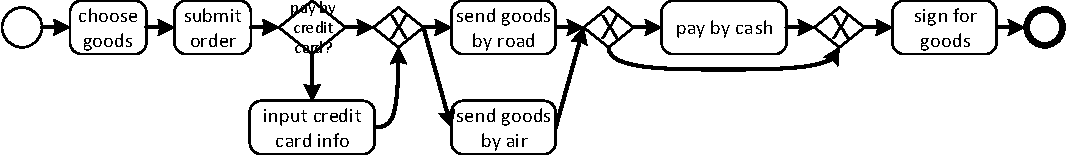
\includegraphics[width=1.0\textwidth]{basic_causal_drawback}
  \caption{含有不同因果关系的在线购物BPMN模型\label{fig:basic_causal_drawback}}
\end{figure}

\begin{example}\label{ex:basic_causal_drawback}
图\ref{fig:basic_causal_drawback}展示了一个在线购物的BPMN模型\footnote{BPMN是一种工作流建模语言,请参见:http://www.bpmn.org/}。在这个模型中,当任务“choose goods”被执行后,任务“submit order”可以被执行,然后任务“send goods by road”和任务“send goods by air”的其中之一可以被执行。显然,任务“choose goods”和任务“submit order”、任务“submit order”和任务“send goods by road”都满足因果关系。然而,这两组因果关系是不完全相同的。当任务“choose goods”被执行后,任务“submit order”一定会被执行而当任务“submit order”被执行后,任务“send goods by road”却不一定会被执行(因为任务“send goods by air”可能被选择执行)。前文提到的基本因果关系不能表达这类不同,所以需要对因果关系进行精炼。
\end{example}

\begin{figure}[htbp]
  \centering
  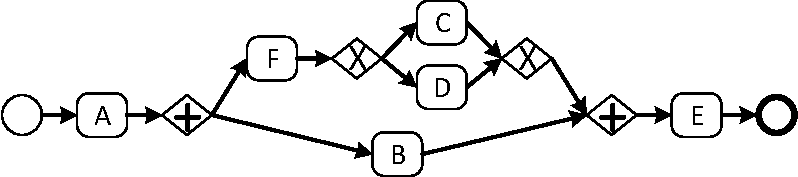
\includegraphics[width=0.8\textwidth]{basic_concurrency_drawback}
  \caption{含有不同并行关系的BPMN模型\label{fig:basic_concurrency_drawback}}
\end{figure}

\begin{example}\label{ex:basic_concurrency_drawback}
图\ref{fig:basic_concurrency_drawback}展示了一个含有并行结构的BPMN模型。在这个模型中,任务“B”和任务“C”可以被并行地执行但当任务“B”被执行时,任务“C”不一定会在同一个执行实例中被执行(因为任务“D”可能被选择执行)。同时,任务“B”和任务“F”也可以被并行地执行而且当任务“B”被执行时,任务“F”一定会在同一个执行实例中被执行。前文提到的基本并行关系不能表达这类不同,所以需要对并行关系进行精炼。
\end{example}

过程模型的任务间不确定性精炼有序关系(以下简称“精炼有序关系”)可以用来刻画过程的行为语义,从而被用于过程模型的检索,即提供一个查询模型$M$和一个过程模型集合$C$,从$C$中查找和$M$行为一致或者最相似的模型。由于本文的方法对过程模型进行了唯一的刻画,所以在检索过程中可以设置不同的粒度以检索符合实际要求的模型。除此之外,精炼有序关系还可以应用于过程模型的符合性检测、相似性度量等领域。

\begin{figure}[htbp]
  \centering
  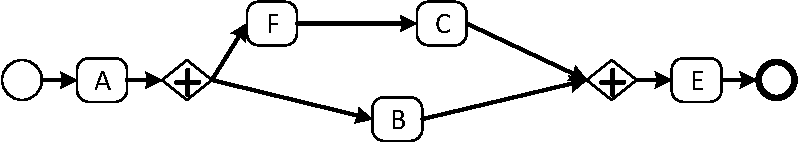
\includegraphics[width=0.8\textwidth]{basic_concurrency_drawback_compare}
  \caption{由图\ref{fig:basic_concurrency_drawback}改造得到的BPMN模型\label{fig:basic_concurrency_drawback_compare}}
\end{figure}

\begin{example}\label{ex:basic_concurrency_drawback_compare}
考虑图\ref{fig:basic_concurrency_drawback}和图\ref{fig:basic_concurrency_drawback_compare}中的模型,当检索满足条件“任务`F'和任务`C'满足因果关系且任务`B'和任务`C'满足并行关系”的模型时,两个模型都符合检索条件。另一方面,将检索条件更改为“任务`F'和任务`C'满足因果关系,且当任务`F'被执行时,任务`C'一定在同一个执行实例中被执行,同时当任务`C'被执行时,任务`F'一定在同一个执行实例中被执行;任务`B'和任务`C'满足并行关系,当任务`B'被执行时,任务`C'一定在同一个执行实例中被执行,同时当任务`C'被执行时,任务`B'一定在同一个执行实例中被执行”时,只有图\ref{fig:basic_concurrency_drawback_compare}中的模型符合条件。显然,精炼后的任务间有序关系能够更加精确地刻画过程模型的行为语义。类似的,这种精炼后的刻画方法可以被当作业务规则用于过程模型的符合性检测。
\end{example}

Jin等人已经提出了一种精炼有序关系RORU及其计算方法\cite{jin2014computing},本文重点对其进行了研究。针对该方法存在的问题,本文提出了改进方案,将新的方法命名为扩展的任务间不确定性精炼有序关系(Extended Refined Ordering Relations with Uncertainty,简称ExRORU)。由于ExRORU是一种刻画过程行为语义的方法,因此在实验过程中,本文将ExRORU与基于行为语义的过程特征刻画算法和过程相似性度量算法进行比较。

\section{预备知识}\label{sec:preliminaries}
本节介绍论文中需要用到的预备知识,其中\ref{subsec:petrinet}介绍Petri网,\ref{subsec:workflow_net}介绍工作流网及相关概念,\ref{subsec:process_run}和\ref{subsec:cpu}分别介绍过程流和完全前缀展开。

\subsection{Petri网}\label{subsec:petrinet}
业务过程建模给业务过程分析人员提供了建立过程模型并分析它们的能力,有许多论著和建模工具对其进行详尽地描述和实现。建模语言是业务过程建模中的核心部分,目前的建模语言包括但不限于:Petri网、EPC(Event-driven process chain,事件驱动过程链)、BPMN(Business Process Model and Notation,业务过程建模符号)、BPEL(Business Process Execution Language,业务过程执行语言)、UML(Unified Modeling Language,统一建模语言)、APROMORE\cite{la2011apromore}。

Petri网是一种有向二分图,于1960年代由Carl Adam Petri发明\cite{petri1962kommunikation},适合于描述含有异步、并发过程的系统。Petri网既有严格的数学表述方式,也有良好的图形化基础。本文使用Petri网作为建模语言。

\begin{definition}[Petri网]\label{def:petrinet}
Petri网是一个三元组$N=(P,T,F)$,其中:
  \begin{itemize}
  	\item[-] $P$是库所的有限集合;
  	\item[-] $T$是变迁的有限集合;
  	\item[-] $P\cap T=\emptyset$且$T\cap P=\emptyset$;
  	\item[-] $F\subseteq(P\times T)\cup(T\times P)$是边的集合。
  \end{itemize}
\end{definition}

\begin{definition}[标识Petri网]\label{def:marked_petrinet}
标识Petri网是一个二元组$(N,s)$,其中$N=(P,T,F)$是一个Petri网,$s:P\rightarrow\mathbb{N}$是一个函数,表示网的标识。所有标识Petri网的集合记作$\mathcal{N}$。
\end{definition}

令$N=(P,T,F)$是一个Petri网。$P\cup T$中的元素称作节点。节点$x$是节点$y$的输入节点,当且仅当$(x,y)\in F$;节点$x$是节点$y$的输出节点,当且仅当$(y,x)\in F$。对于任意节点$x\in P\cup T$,$x$的前集$\bullet x=\{y|(y,x)\in F\}$,$x$的后集$x\bullet=\{y|(x,y)\in F\}$。

\begin{figure}[htbp]
  \centering
  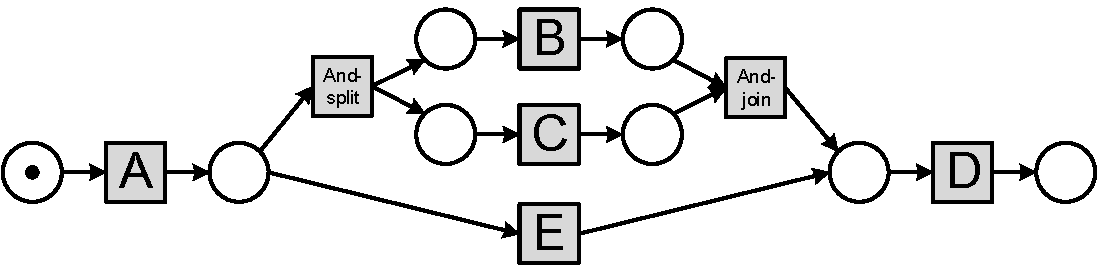
\includegraphics[width=0.8\textwidth]{petri_net_example}
  \caption{标识Petri网示例\label{fig:petri_net_example}}
\end{figure}

图\ref{fig:petri_net_example}展示了一个由8个库所和7个变迁组成的Petri网。变迁$A$有一个输入库所和一个输出库所,变迁$AND$-$split$有一个输入库所和两个输出库所,变迁$AND$-$join$有两个输入库所和一个输出库所。变迁$A$的输入库所中的黑点表示一个托肯(token),这个托肯即为该Petri网的初始标识。该Petri网的行为由如下发生规则定义。

\begin{definition}[发生规则]\label{def:firing_rule}
令$\Sigma=(N=(P,T,F),M_{0})$是一个Petri网系统:
  \begin{itemize}
  	\item[-] 变迁$t\in T$被使能,记作$(N,s)[t\rangle$,当且仅当$\bullet t\leq s$;
  	\item[-] 发生规则$\_[\_\rangle\_\subseteq\mathcal{N}\times T\times\mathcal{N}$是满足如下条件的最小关系:\\$\forall (N=(P,T,F),s)\in\mathcal{N},\forall t\in T:(N,s)[t\rangle\Rightarrow(N,s)[t\rangle(N,s-\bullet t+t\bullet)$。
  \end{itemize}
\end{definition}

在图\ref{fig:petri_net_example}的标识Petri网(源库所有一个托肯)中,变迁$A$被使能。当变迁$A$发生后,会将其输入库所中的托肯移除,在其输出库所中加入一个托肯,如图\ref{fig:petri_net_example_fire1}所示。此时,变迁$E$和变迁$AND$-$split$都被使能。虽然两者都被使能,但是只有一个能够发生,因为变迁$E$和变迁$AND$-$split$此时会竞争唯一的托肯。如果变迁$AND$-$split$发生,会消耗其输入库所的托肯并在两个输出库所中各生成一个托肯,如图\ref{fig:petri_net_example_fire2}所示。

\begin{figure}[htbp]
  \centering
  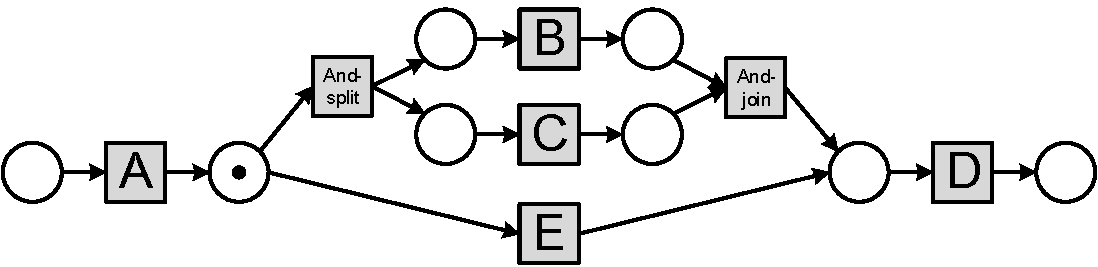
\includegraphics[width=0.8\textwidth]{petri_net_example_fire1}
  \caption{变迁$A$发生后的标识Petri网\label{fig:petri_net_example_fire1}}
\end{figure}

\begin{figure}[htbp]
  \centering
  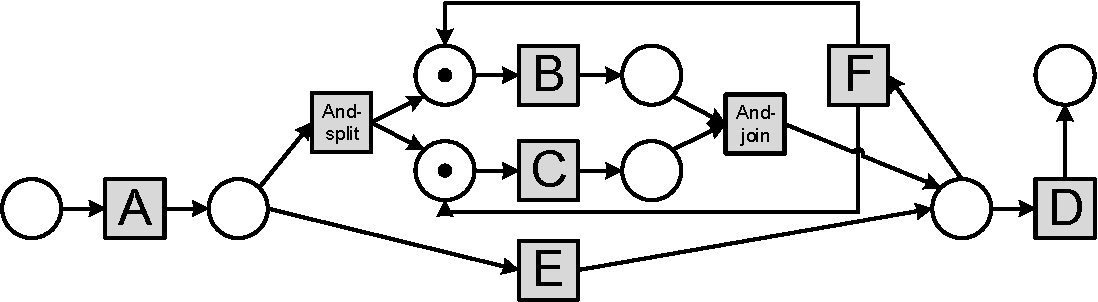
\includegraphics[width=0.8\textwidth]{petri_net_example_fire2}
  \caption{变迁$AND$-$split$发生后的标识Petri网\label{fig:petri_net_example_fire2}}
\end{figure}

\begin{definition}[可达标识]\label{def:reachable_markings}
令$(N,s_{0})\in\mathcal{N}$是一个标识Petri网。标识$s$从初始标识$s_{0}$可达,当且仅当存在一条变迁序列,其变迁依次发生使标识$s_{0}$变为$s$。$(N,s_{0})$所有可达标识的集合记作$[N,s_{0}\rangle$。
\end{definition}

图\ref{fig:petri_net_example}中的标识Petri网有八个可达标识。本文用如下方式描述到达某个可达标识的变迁发生序列。令$A$为标签集合。由$A$内元素组成的长度为$n\in\mathbb{N}$的序列是一个函数$\sigma:\{0,...,n-1\}\rightarrow A$。长度为0的序列称作空序列,记作$\varepsilon$。为了便于理解,一个长度大于0的序列通常简写为函数的值序列。例如,序列$\sigma=\{(0,a),(1,a),(2,b)\}$简写为$aab$。由$A$内元素组成的任意长度的所有序列集合记作$A^{*}$。

\begin{definition}[发生序列]\label{def:firing_sequence}
令$(N=(P,T,F),s_{0})$是一个标识Petri网。序列$\sigma\in T^{*}$是$(N,s_{0})$的一条发生序列当且仅当对于某个自然数$n\in\mathbb{N}$,存在标识$s_{1},...,s_{n}$和变迁$t_{1},...,t_{n}\in T$,使得$\sigma=t_{1}...t_{n}$,且对于所有满足$0\leq i\leq n$的$i$,$(N,s_{i})[t_{i+1}\rangle$且$s_{i+1}=s_{i}-\bullet t_{i+1}+t_{i+1}\bullet$。($n=0$隐含$\sigma=\varepsilon$,$\varepsilon$是$(N,s_{0})$的发生序列。)序列$\sigma$在标识$s_{0}$下可发生,记作$(N,s_{0})[\sigma\rangle$。序列$\sigma$发生后得到标识$s_{n}$,记作$(N,s_{0})[\sigma\rangle(N,s_{n})$。
\end{definition}

\begin{definition}[连通性]\label{def:connectedness}
网$N=(P,T,F)$是弱连通的,或者简称连通的,当且仅当对于任意两个节点$x,y\in P\cup T$,$x(F\cup F^{-1})y$,其中$R^{-1}$是关系$R$的逆,$R^{*}$是关系$R$的自反传递闭包。网$N$是强联通的,当且仅当对于任意两个节点$x,y\in P\cup T$,$xF^{*}y$。
\end{definition}

图\ref{fig:petri_net_example}中的标识Petri网是连通的,但不是强连通的,例如没有从汇库所到源库所的有向路径,也没有从变迁$D$到变迁$A$的有向路径。

\begin{definition}[有界性、安全性]\label{def:boundedness_safeness}
标识Petri网$(N=(P,T,F),s)$是有界的,当且仅当可达标识集合$[N,s\rangle$是有穷的。$(N,s)$是安全的,当且仅当$\forall s'\in[N,s\rangle,\forall p\in P,s.t.~s'(p)\leq 1$。显然,安全性隐含了有界性。
\end{definition}

图\ref{fig:petri_net_example}中的标识Petri网是安全的(也是有界的),因为它的八个可达标识中没有库所会包含超过一个托肯。

\begin{definition}[死变迁,活性]\label{def:dead_transition}
令$(N=(P,T,F),s)$是一个标识Petri网。变迁$t\in T$是死变迁当且仅当$\nexists s'\in[N,s\rangle,s.t.~(N,s')[t\rangle$。$(N,s)$是活的,当且仅当$\forall s'\in[N,s\rangle,\forall t\in T,s.t.~\exists s'\in[N,s'\rangle,(N,s')[t\rangle$。显然,活性隐含不存在死变迁。
\end{definition}

图\ref{fig:petri_net_example}中的标识Petri网的所有变迁都不是死变迁。但是它不是活的,因为它无法使每个变迁不断地发生。

\subsection{工作流网}\label{subsec:workflow_net}

\subsection{过程流}\label{subsec:process_run}

\subsection{完全前缀展开}\label{subsec:cpu}

\section{论文的主要贡献}\label{sec:contribution}

\section{论文章节安排}\label{sec:structure}